\documentclass[twoside]{book}

% Packages required by doxygen
\usepackage{fixltx2e}
\usepackage{calc}
\usepackage{doxygen}
\usepackage[export]{adjustbox} % also loads graphicx
\usepackage{graphicx}
\usepackage[utf8]{inputenc}
\usepackage{makeidx}
\usepackage{multicol}
\usepackage{multirow}
\PassOptionsToPackage{warn}{textcomp}
\usepackage{textcomp}
\usepackage[nointegrals]{wasysym}
\usepackage[table]{xcolor}

% NLS support packages
\usepackage{polski}
\usepackage[T1]{fontenc}

% Font selection
\usepackage[T1]{fontenc}
\usepackage[scaled=.90]{helvet}
\usepackage{courier}
\usepackage{amssymb}
\usepackage{sectsty}
\renewcommand{\familydefault}{\sfdefault}
\allsectionsfont{%
  \fontseries{bc}\selectfont%
  \color{darkgray}%
}
\renewcommand{\DoxyLabelFont}{%
  \fontseries{bc}\selectfont%
  \color{darkgray}%
}
\newcommand{\+}{\discretionary{\mbox{\scriptsize$\hookleftarrow$}}{}{}}

% Page & text layout
\usepackage{geometry}
\geometry{%
  a4paper,%
  top=2.5cm,%
  bottom=2.5cm,%
  left=2.5cm,%
  right=2.5cm%
}
\tolerance=750
\hfuzz=15pt
\hbadness=750
\setlength{\emergencystretch}{15pt}
\setlength{\parindent}{0cm}
\setlength{\parskip}{3ex plus 2ex minus 2ex}
\makeatletter
\renewcommand{\paragraph}{%
  \@startsection{paragraph}{4}{0ex}{-1.0ex}{1.0ex}{%
    \normalfont\normalsize\bfseries\SS@parafont%
  }%
}
\renewcommand{\subparagraph}{%
  \@startsection{subparagraph}{5}{0ex}{-1.0ex}{1.0ex}{%
    \normalfont\normalsize\bfseries\SS@subparafont%
  }%
}
\makeatother

% Headers & footers
\usepackage{fancyhdr}
\pagestyle{fancyplain}
\fancyhead[LE]{\fancyplain{}{\bfseries\thepage}}
\fancyhead[CE]{\fancyplain{}{}}
\fancyhead[RE]{\fancyplain{}{\bfseries\leftmark}}
\fancyhead[LO]{\fancyplain{}{\bfseries\rightmark}}
\fancyhead[CO]{\fancyplain{}{}}
\fancyhead[RO]{\fancyplain{}{\bfseries\thepage}}
\fancyfoot[LE]{\fancyplain{}{}}
\fancyfoot[CE]{\fancyplain{}{}}
\fancyfoot[RE]{\fancyplain{}{\bfseries\scriptsize Wygenerowano przez Doxygen }}
\fancyfoot[LO]{\fancyplain{}{\bfseries\scriptsize Wygenerowano przez Doxygen }}
\fancyfoot[CO]{\fancyplain{}{}}
\fancyfoot[RO]{\fancyplain{}{}}
\renewcommand{\footrulewidth}{0.4pt}
\renewcommand{\chaptermark}[1]{%
  \markboth{#1}{}%
}
\renewcommand{\sectionmark}[1]{%
  \markright{\thesection\ #1}%
}

% Indices & bibliography
\usepackage{natbib}
\usepackage[titles]{tocloft}
\setcounter{tocdepth}{3}
\setcounter{secnumdepth}{5}
\makeindex

% Hyperlinks (required, but should be loaded last)
\usepackage{ifpdf}
\ifpdf
  \usepackage[pdftex,pagebackref=true]{hyperref}
\else
  \usepackage[ps2pdf,pagebackref=true]{hyperref}
\fi
\hypersetup{%
  colorlinks=true,%
  linkcolor=blue,%
  citecolor=blue,%
  unicode%
}

% Custom commands
\newcommand{\clearemptydoublepage}{%
  \newpage{\pagestyle{empty}\cleardoublepage}%
}

\usepackage{caption}
\captionsetup{labelsep=space,justification=centering,font={bf},singlelinecheck=off,skip=4pt,position=top}

%===== C O N T E N T S =====

\begin{document}

% Titlepage & ToC
\hypersetup{pageanchor=false,
             bookmarksnumbered=true,
             pdfencoding=unicode
            }
\pagenumbering{roman}
\begin{titlepage}
\vspace*{7cm}
\begin{center}%
{\Large Gra Edukacyjan dla dzieci }\\
\vspace*{1cm}
{\large Wygenerowano przez Doxygen 1.8.11}\\
\end{center}
\end{titlepage}
\clearemptydoublepage
\tableofcontents
\clearemptydoublepage
\pagenumbering{arabic}
\hypersetup{pageanchor=true}

%--- Begin generated contents ---
\chapter{Indeks przestrzeni nazw}
\section{Pakiety}
Oto lista pakietów wraz z krótkim opisem (o ile jest dostępny)\+:\begin{DoxyCompactList}
\item\contentsline{section}{\hyperlink{namespace_zdjecia}{Zdjecia} }{\pageref{namespace_zdjecia}}{}
\item\contentsline{section}{\hyperlink{namespace_zdjecia_1_1_properties}{Zdjecia.\+Properties} }{\pageref{namespace_zdjecia_1_1_properties}}{}
\end{DoxyCompactList}

\chapter{Indeks hierarchiczny}
\section{Hierarchia klas}
Ta lista dziedziczenia posortowana jest z grubsza, choć nie całkowicie, alfabetycznie\+:\begin{DoxyCompactList}
\item Form\begin{DoxyCompactList}
\item \contentsline{section}{Zdjecia.\+Form1}{\pageref{class_zdjecia_1_1_form1}}{}
\item \contentsline{section}{Zdjecia.\+Form2}{\pageref{class_zdjecia_1_1_form2}}{}
\end{DoxyCompactList}
\item Panel\begin{DoxyCompactList}
\item \contentsline{section}{Zdjecia.\+My\+Picture\+Box}{\pageref{class_zdjecia_1_1_my_picture_box}}{}
\end{DoxyCompactList}
\item \contentsline{section}{Zdjecia.\+Uzytkownik}{\pageref{class_zdjecia_1_1_uzytkownik}}{}
\end{DoxyCompactList}

\chapter{Indeks klas}
\section{Lista klas}
Tutaj znajdują się klasy, struktury, unie i interfejsy wraz z ich krótkimi opisami\+:\begin{DoxyCompactList}
\item\contentsline{section}{\hyperlink{class_zdjecia_1_1_form1}{Zdjecia.\+Form1} \\*\hyperlink{class_zdjecia_1_1_form1}{Form1} sluzy do wysiwetlania glownego ekranu gry }{\pageref{class_zdjecia_1_1_form1}}{}
\item\contentsline{section}{\hyperlink{class_zdjecia_1_1_form2}{Zdjecia.\+Form2} \\*\hyperlink{class_zdjecia_1_1_form2}{Form2} sluzy do wysiwetlenia ekranu logowania i utworzeniu profilu gracza }{\pageref{class_zdjecia_1_1_form2}}{}
\item\contentsline{section}{\hyperlink{class_zdjecia_1_1_my_picture_box}{Zdjecia.\+My\+Picture\+Box} \\*\hyperlink{class_zdjecia_1_1_my_picture_box}{My\+Picture\+Box} sluzy do wyswietlania obrazkow }{\pageref{class_zdjecia_1_1_my_picture_box}}{}
\item\contentsline{section}{\hyperlink{class_zdjecia_1_1_uzytkownik}{Zdjecia.\+Uzytkownik} \\*\hyperlink{class_zdjecia_1_1_uzytkownik}{Uzytkownik} sluzy do tworzenia profilu uzytkownika }{\pageref{class_zdjecia_1_1_uzytkownik}}{}
\end{DoxyCompactList}

\chapter{Indeks plików}
\section{Lista plików}
Tutaj znajduje się lista wszystkich udokumentowanych plików z ich krótkimi opisami\+:\begin{DoxyCompactList}
\item\contentsline{section}{Zdjecia/\hyperlink{_form1_8cs}{Form1.\+cs} }{\pageref{_form1_8cs}}{}
\item\contentsline{section}{Zdjecia/\hyperlink{_form2_8cs}{Form2.\+cs} }{\pageref{_form2_8cs}}{}
\item\contentsline{section}{Zdjecia/\hyperlink{_my_picture_box_8cs}{My\+Picture\+Box.\+cs} }{\pageref{_my_picture_box_8cs}}{}
\item\contentsline{section}{Zdjecia/\hyperlink{_program_8cs}{Program.\+cs} }{\pageref{_program_8cs}}{}
\item\contentsline{section}{Zdjecia/\hyperlink{_uzytkownik_8cs}{Uzytkownik.\+cs} }{\pageref{_uzytkownik_8cs}}{}
\end{DoxyCompactList}

\chapter{Dokumentacja przestrzeni nazw}
\hypertarget{namespace_zdjecia}{}\section{Dokumentacja przestrzeni nazw Zdjecia}
\label{namespace_zdjecia}\index{Zdjecia@{Zdjecia}}
\subsection*{Przestrzenie nazw}
\begin{DoxyCompactItemize}
\end{DoxyCompactItemize}
\subsection*{Komponenty}
\begin{DoxyCompactItemize}
\item 
class \hyperlink{class_zdjecia_1_1_form1}{Form1}
\begin{DoxyCompactList}\small\item\em \hyperlink{class_zdjecia_1_1_form1}{Form1} sluzy do wysiwetlania glownego ekranu gry. \end{DoxyCompactList}\item 
class \hyperlink{class_zdjecia_1_1_form2}{Form2}
\begin{DoxyCompactList}\small\item\em \hyperlink{class_zdjecia_1_1_form2}{Form2} sluzy do wysiwetlenia ekranu logowania i utworzeniu profilu gracza. \end{DoxyCompactList}\item 
class \hyperlink{class_zdjecia_1_1_my_picture_box}{My\+Picture\+Box}
\begin{DoxyCompactList}\small\item\em \hyperlink{class_zdjecia_1_1_my_picture_box}{My\+Picture\+Box} sluzy do wyswietlania obrazkow. \end{DoxyCompactList}\item 
class {\bfseries Program}
\begin{DoxyCompactList}\small\item\em Program sluzy do uruchamiania gry. \end{DoxyCompactList}\item 
class \hyperlink{class_zdjecia_1_1_uzytkownik}{Uzytkownik}
\begin{DoxyCompactList}\small\item\em \hyperlink{class_zdjecia_1_1_uzytkownik}{Uzytkownik} sluzy do tworzenia profilu uzytkownika. \end{DoxyCompactList}\end{DoxyCompactItemize}

\hypertarget{namespace_zdjecia_1_1_properties}{}\section{Dokumentacja przestrzeni nazw Zdjecia.\+Properties}
\label{namespace_zdjecia_1_1_properties}\index{Zdjecia.\+Properties@{Zdjecia.\+Properties}}
\subsection*{Komponenty}
\begin{DoxyCompactItemize}
\item 
class {\bfseries Resources}
\begin{DoxyCompactList}\small\item\em A strongly-\/typed resource class, for looking up localized strings, etc. \end{DoxyCompactList}\item 
class {\bfseries Settings}
\end{DoxyCompactItemize}

\chapter{Dokumentacja klas}
\hypertarget{class_zdjecia_1_1_form1}{}\section{Dokumentacja klasy Zdjecia.\+Form1}
\label{class_zdjecia_1_1_form1}\index{Zdjecia.\+Form1@{Zdjecia.\+Form1}}


\hyperlink{class_zdjecia_1_1_form1}{Form1} sluzy do wysiwetlania glownego ekranu gry.  


Diagram dziedziczenia dla Zdjecia.\+Form1\begin{figure}[H]
\begin{center}
\leavevmode
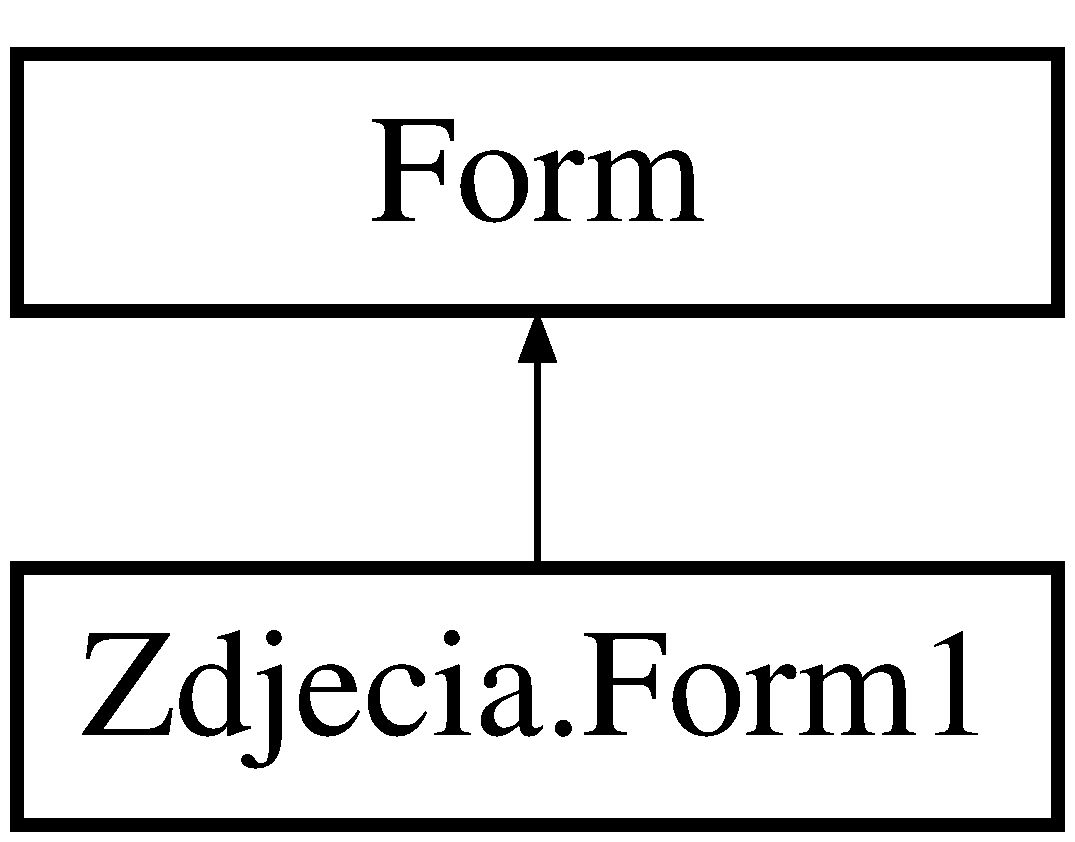
\includegraphics[height=2.000000cm]{class_zdjecia_1_1_form1}
\end{center}
\end{figure}
\subsection*{Metody publiczne}
\begin{DoxyCompactItemize}
\item 
\hyperlink{class_zdjecia_1_1_form1_aed2fd4d34288702c4cd81d0b1353c218}{Form1} ()\hypertarget{class_zdjecia_1_1_form1_aed2fd4d34288702c4cd81d0b1353c218}{}\label{class_zdjecia_1_1_form1_aed2fd4d34288702c4cd81d0b1353c218}

\begin{DoxyCompactList}\small\item\em konstruktor klasy Form 1 \end{DoxyCompactList}\end{DoxyCompactItemize}
\subsection*{Atrybuty publiczne}
\begin{DoxyCompactItemize}
\item 
System.\+Windows.\+Forms.\+Label {\bfseries label1}\hypertarget{class_zdjecia_1_1_form1_a15aa615fa1a5034315d622c128761a8f}{}\label{class_zdjecia_1_1_form1_a15aa615fa1a5034315d622c128761a8f}

\item 
System.\+Windows.\+Forms.\+Label {\bfseries label2}\hypertarget{class_zdjecia_1_1_form1_ae0dc4ff16396e37af41b6b5dd87d63dc}{}\label{class_zdjecia_1_1_form1_ae0dc4ff16396e37af41b6b5dd87d63dc}

\item 
System.\+Windows.\+Forms.\+Text\+Box {\bfseries text\+Box1}\hypertarget{class_zdjecia_1_1_form1_a960517bc88a4fef5ce90604872eb5038}{}\label{class_zdjecia_1_1_form1_a960517bc88a4fef5ce90604872eb5038}

\end{DoxyCompactItemize}
\subsection*{Metody chronione}
\begin{DoxyCompactItemize}
\item 
override void \hyperlink{class_zdjecia_1_1_form1_af0513b0ee9e0807216541866c567c767}{Dispose} (bool disposing)
\begin{DoxyCompactList}\small\item\em Clean up any resources being used. \end{DoxyCompactList}\end{DoxyCompactItemize}


\subsection{Opis szczegółowy}
\hyperlink{class_zdjecia_1_1_form1}{Form1} sluzy do wysiwetlania glownego ekranu gry. 

\subsection{Dokumentacja funkcji składowych}
\index{Zdjecia\+::\+Form1@{Zdjecia\+::\+Form1}!Dispose@{Dispose}}
\index{Dispose@{Dispose}!Zdjecia\+::\+Form1@{Zdjecia\+::\+Form1}}
\subsubsection[{\texorpdfstring{Dispose(bool disposing)}{Dispose(bool disposing)}}]{\setlength{\rightskip}{0pt plus 5cm}override void Zdjecia.\+Form1.\+Dispose (
\begin{DoxyParamCaption}
\item[{bool}]{disposing}
\end{DoxyParamCaption}
)\hspace{0.3cm}{\ttfamily [protected]}}\hypertarget{class_zdjecia_1_1_form1_af0513b0ee9e0807216541866c567c767}{}\label{class_zdjecia_1_1_form1_af0513b0ee9e0807216541866c567c767}


Clean up any resources being used. 


\begin{DoxyParams}{Parametry}
{\em disposing} & true if managed resources should be disposed; otherwise, false.\\
\hline
\end{DoxyParams}


Dokumentacja dla tej klasy została wygenerowana z plików\+:\begin{DoxyCompactItemize}
\item 
Zdjecia/\hyperlink{_form1_8cs}{Form1.\+cs}\item 
Zdjecia/Form1.\+Designer.\+cs\end{DoxyCompactItemize}

\hypertarget{class_zdjecia_1_1_form2}{}\section{Dokumentacja klasy Zdjecia.\+Form2}
\label{class_zdjecia_1_1_form2}\index{Zdjecia.\+Form2@{Zdjecia.\+Form2}}


\hyperlink{class_zdjecia_1_1_form2}{Form2} sluzy do wysiwetlenia ekranu logowania i utworzeniu profilu gracza.  


Diagram dziedziczenia dla Zdjecia.\+Form2\begin{figure}[H]
\begin{center}
\leavevmode
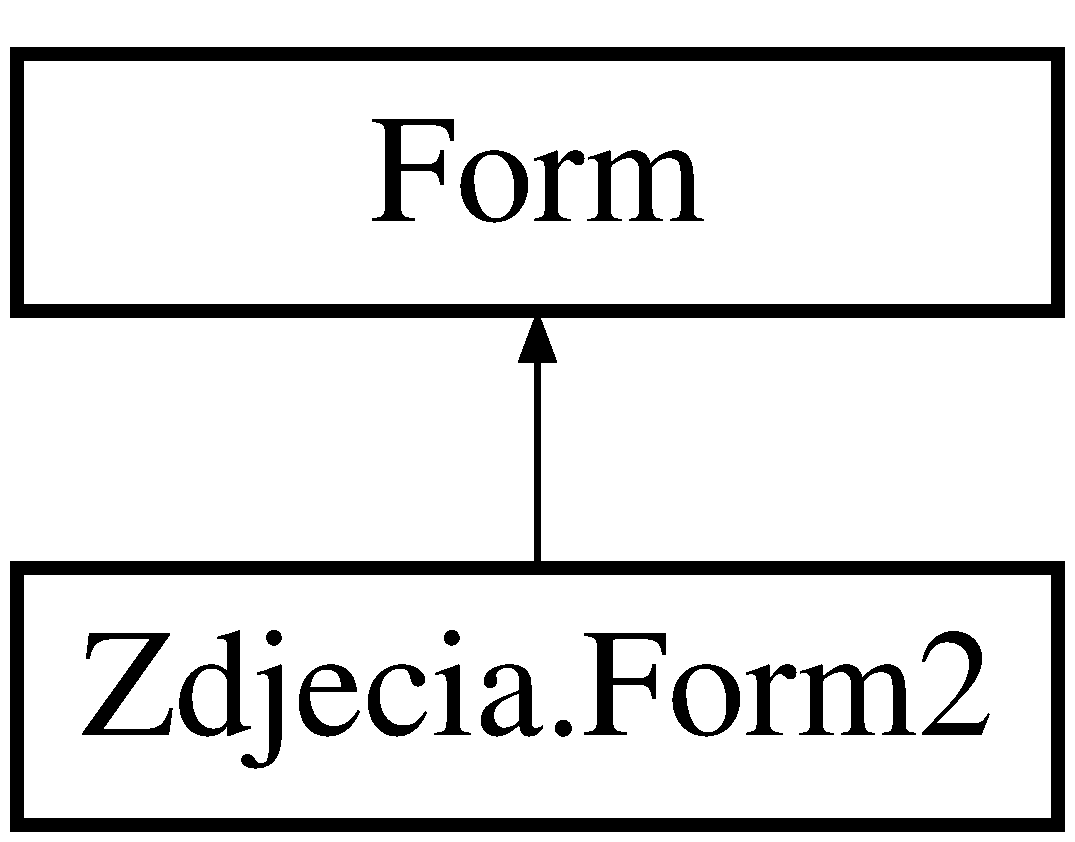
\includegraphics[height=2.000000cm]{class_zdjecia_1_1_form2}
\end{center}
\end{figure}
\subsection*{Metody publiczne}
\begin{DoxyCompactItemize}
\item 
\hyperlink{class_zdjecia_1_1_form2_a42e414daffdb6ffe10502528c6c96380}{Form2} (\hyperlink{class_zdjecia_1_1_form1}{Form1} forma1)\hypertarget{class_zdjecia_1_1_form2_a42e414daffdb6ffe10502528c6c96380}{}\label{class_zdjecia_1_1_form2_a42e414daffdb6ffe10502528c6c96380}

\begin{DoxyCompactList}\small\item\em konstruktor klasy \hyperlink{class_zdjecia_1_1_form2}{Form2} \end{DoxyCompactList}\end{DoxyCompactItemize}
\subsection*{Metody chronione}
\begin{DoxyCompactItemize}
\item 
override void \hyperlink{class_zdjecia_1_1_form2_ad08c002d9f33b53ceb56826d732ce8b8}{Dispose} (bool disposing)
\begin{DoxyCompactList}\small\item\em Clean up any resources being used. \end{DoxyCompactList}\end{DoxyCompactItemize}


\subsection{Opis szczegółowy}
\hyperlink{class_zdjecia_1_1_form2}{Form2} sluzy do wysiwetlenia ekranu logowania i utworzeniu profilu gracza. 

\subsection{Dokumentacja funkcji składowych}
\index{Zdjecia\+::\+Form2@{Zdjecia\+::\+Form2}!Dispose@{Dispose}}
\index{Dispose@{Dispose}!Zdjecia\+::\+Form2@{Zdjecia\+::\+Form2}}
\subsubsection[{\texorpdfstring{Dispose(bool disposing)}{Dispose(bool disposing)}}]{\setlength{\rightskip}{0pt plus 5cm}override void Zdjecia.\+Form2.\+Dispose (
\begin{DoxyParamCaption}
\item[{bool}]{disposing}
\end{DoxyParamCaption}
)\hspace{0.3cm}{\ttfamily [protected]}}\hypertarget{class_zdjecia_1_1_form2_ad08c002d9f33b53ceb56826d732ce8b8}{}\label{class_zdjecia_1_1_form2_ad08c002d9f33b53ceb56826d732ce8b8}


Clean up any resources being used. 


\begin{DoxyParams}{Parametry}
{\em disposing} & true if managed resources should be disposed; otherwise, false.\\
\hline
\end{DoxyParams}


Dokumentacja dla tej klasy została wygenerowana z plików\+:\begin{DoxyCompactItemize}
\item 
Zdjecia/\hyperlink{_form2_8cs}{Form2.\+cs}\item 
Zdjecia/Form2.\+Designer.\+cs\end{DoxyCompactItemize}

\hypertarget{class_zdjecia_1_1_my_picture_box}{}\section{Dokumentacja klasy Zdjecia.\+My\+Picture\+Box}
\label{class_zdjecia_1_1_my_picture_box}\index{Zdjecia.\+My\+Picture\+Box@{Zdjecia.\+My\+Picture\+Box}}


\hyperlink{class_zdjecia_1_1_my_picture_box}{My\+Picture\+Box} sluzy do wyswietlania obrazkow.  


Diagram dziedziczenia dla Zdjecia.\+My\+Picture\+Box\begin{figure}[H]
\begin{center}
\leavevmode
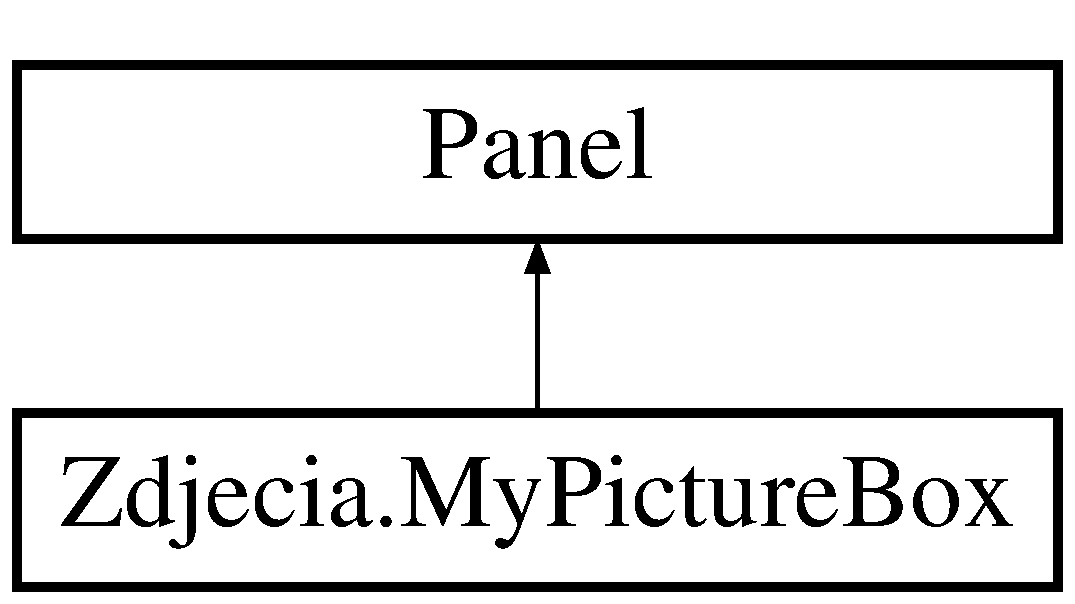
\includegraphics[height=2.000000cm]{class_zdjecia_1_1_my_picture_box}
\end{center}
\end{figure}
\subsection*{Metody publiczne}
\begin{DoxyCompactItemize}
\item 
\hyperlink{class_zdjecia_1_1_my_picture_box_a90cd7b95014724ea93c1cecb0f959c8f}{My\+Picture\+Box} ()\hypertarget{class_zdjecia_1_1_my_picture_box_a90cd7b95014724ea93c1cecb0f959c8f}{}\label{class_zdjecia_1_1_my_picture_box_a90cd7b95014724ea93c1cecb0f959c8f}

\begin{DoxyCompactList}\small\item\em konstruktor odpowiadajacy za tworzenie obiektu \hyperlink{class_zdjecia_1_1_my_picture_box}{My\+Picture\+Box} oraz kontrolki \end{DoxyCompactList}\item 
void \hyperlink{class_zdjecia_1_1_my_picture_box_ae82545a339de3030575a0d72b3bb3def}{Load\+From\+File} (string txt)\hypertarget{class_zdjecia_1_1_my_picture_box_ae82545a339de3030575a0d72b3bb3def}{}\label{class_zdjecia_1_1_my_picture_box_ae82545a339de3030575a0d72b3bb3def}

\begin{DoxyCompactList}\small\item\em funkcja odpowiadajaca za wczytywanie z pliku \end{DoxyCompactList}\item 
void {\bfseries Zoom\+In} ()\hypertarget{class_zdjecia_1_1_my_picture_box_a06be7eb1a2f5ff281adcec73eb7adcbc}{}\label{class_zdjecia_1_1_my_picture_box_a06be7eb1a2f5ff281adcec73eb7adcbc}

\item 
void {\bfseries Zoom\+Out} ()\hypertarget{class_zdjecia_1_1_my_picture_box_a0c974a3a80623937181407146427db00}{}\label{class_zdjecia_1_1_my_picture_box_a0c974a3a80623937181407146427db00}

\end{DoxyCompactItemize}


\subsection{Opis szczegółowy}
\hyperlink{class_zdjecia_1_1_my_picture_box}{My\+Picture\+Box} sluzy do wyswietlania obrazkow. 

Dokumentacja dla tej klasy została wygenerowana z pliku\+:\begin{DoxyCompactItemize}
\item 
Zdjecia/\hyperlink{_my_picture_box_8cs}{My\+Picture\+Box.\+cs}\end{DoxyCompactItemize}

\hypertarget{class_zdjecia_1_1_uzytkownik}{}\section{Dokumentacja klasy Zdjecia.\+Uzytkownik}
\label{class_zdjecia_1_1_uzytkownik}\index{Zdjecia.\+Uzytkownik@{Zdjecia.\+Uzytkownik}}


\hyperlink{class_zdjecia_1_1_uzytkownik}{Uzytkownik} sluzy do tworzenia profilu uzytkownika.  


\subsection*{Metody publiczne}
\begin{DoxyCompactItemize}
\item 
\hyperlink{class_zdjecia_1_1_uzytkownik_aae2542fc4872b1d3fcb76477433fad49}{Uzytkownik} (string Imie, string plec, int wiek)\hypertarget{class_zdjecia_1_1_uzytkownik_aae2542fc4872b1d3fcb76477433fad49}{}\label{class_zdjecia_1_1_uzytkownik_aae2542fc4872b1d3fcb76477433fad49}

\begin{DoxyCompactList}\small\item\em konstruktor odpowiadajacy za tworzenie nowego uzytkownika \end{DoxyCompactList}\end{DoxyCompactItemize}


\subsection{Opis szczegółowy}
\hyperlink{class_zdjecia_1_1_uzytkownik}{Uzytkownik} sluzy do tworzenia profilu uzytkownika. 

Dokumentacja dla tej klasy została wygenerowana z pliku\+:\begin{DoxyCompactItemize}
\item 
Zdjecia/\hyperlink{_uzytkownik_8cs}{Uzytkownik.\+cs}\end{DoxyCompactItemize}

\chapter{Dokumentacja plików}
\hypertarget{_form1_8cs}{}\section{Dokumentacja pliku Zdjecia/\+Form1.cs}
\label{_form1_8cs}\index{Zdjecia/\+Form1.\+cs@{Zdjecia/\+Form1.\+cs}}
\subsection*{Komponenty}
\begin{DoxyCompactItemize}
\item 
class \hyperlink{class_zdjecia_1_1_form1}{Zdjecia.\+Form1}
\begin{DoxyCompactList}\small\item\em \hyperlink{class_zdjecia_1_1_form1}{Form1} sluzy do wysiwetlania glownego ekranu gry. \end{DoxyCompactList}\end{DoxyCompactItemize}
\subsection*{Przestrzenie nazw}
\begin{DoxyCompactItemize}
\end{DoxyCompactItemize}


\subsection{Opis szczegółowy}
/ /$\ast$$\ast$ 
\hypertarget{_form2_8cs}{}\section{Dokumentacja pliku Zdjecia/\+Form2.cs}
\label{_form2_8cs}\index{Zdjecia/\+Form2.\+cs@{Zdjecia/\+Form2.\+cs}}
\subsection*{Komponenty}
\begin{DoxyCompactItemize}
\item 
class \hyperlink{class_zdjecia_1_1_form2}{Zdjecia.\+Form2}
\begin{DoxyCompactList}\small\item\em \hyperlink{class_zdjecia_1_1_form2}{Form2} sluzy do wysiwetlenia ekranu logowania i utworzeniu profilu gracza. \end{DoxyCompactList}\end{DoxyCompactItemize}
\subsection*{Przestrzenie nazw}
\begin{DoxyCompactItemize}
\end{DoxyCompactItemize}


\subsection{Opis szczegółowy}
/ /$\ast$$\ast$ 
\hypertarget{_my_picture_box_8cs}{}\section{Dokumentacja pliku Zdjecia/\+My\+Picture\+Box.cs}
\label{_my_picture_box_8cs}\index{Zdjecia/\+My\+Picture\+Box.\+cs@{Zdjecia/\+My\+Picture\+Box.\+cs}}
\subsection*{Komponenty}
\begin{DoxyCompactItemize}
\item 
class \hyperlink{class_zdjecia_1_1_my_picture_box}{Zdjecia.\+My\+Picture\+Box}
\begin{DoxyCompactList}\small\item\em \hyperlink{class_zdjecia_1_1_my_picture_box}{My\+Picture\+Box} sluzy do wyswietlania obrazkow. \end{DoxyCompactList}\end{DoxyCompactItemize}
\subsection*{Przestrzenie nazw}
\begin{DoxyCompactItemize}
\end{DoxyCompactItemize}


\subsection{Opis szczegółowy}
/ /$\ast$$\ast$ 
\hypertarget{_program_8cs}{}\section{Dokumentacja pliku Zdjecia/\+Program.cs}
\label{_program_8cs}\index{Zdjecia/\+Program.\+cs@{Zdjecia/\+Program.\+cs}}
\subsection*{Komponenty}
\begin{DoxyCompactItemize}
\item 
class {\bfseries Zdjecia.\+Program}
\begin{DoxyCompactList}\small\item\em Program sluzy do uruchamiania gry. \end{DoxyCompactList}\end{DoxyCompactItemize}
\subsection*{Przestrzenie nazw}
\begin{DoxyCompactItemize}
\end{DoxyCompactItemize}


\subsection{Opis szczegółowy}
/ /$\ast$$\ast$ 
\hypertarget{_uzytkownik_8cs}{}\section{Dokumentacja pliku Zdjecia/\+Uzytkownik.cs}
\label{_uzytkownik_8cs}\index{Zdjecia/\+Uzytkownik.\+cs@{Zdjecia/\+Uzytkownik.\+cs}}
\subsection*{Komponenty}
\begin{DoxyCompactItemize}
\item 
class \hyperlink{class_zdjecia_1_1_uzytkownik}{Zdjecia.\+Uzytkownik}
\begin{DoxyCompactList}\small\item\em \hyperlink{class_zdjecia_1_1_uzytkownik}{Uzytkownik} sluzy do tworzenia profilu uzytkownika. \end{DoxyCompactList}\end{DoxyCompactItemize}
\subsection*{Przestrzenie nazw}
\begin{DoxyCompactItemize}
\end{DoxyCompactItemize}


\subsection{Opis szczegółowy}
/ /$\ast$$\ast$ 
%--- End generated contents ---

% Index
\backmatter
\newpage
\phantomsection
\clearemptydoublepage
\addcontentsline{toc}{chapter}{Indeks}
\printindex

\end{document}
